%%%%%%%%%%%%%%%%%%%%%%%%%%%%%%%%%%%%%%%%%%%%%%%%%%%%%%%%%%%%%%
%% LaTeX template for the science justification to be       %%
%%       submitted as part of an ALMA proposal.             %%
%%                                                          %%
%%                      ALMA Cycle 2                        %%
%%                                                          %%
%%%%%%%%%%%%%%%%%%%%%%%%%%%%%%%%%%%%%%%%%%%%%%%%%%%%%%%%%%%%%%

%%%%%%%%%%%%%%%%%%%%%%%%%%%%%%%%%%%%%%%%%%%%%%%%%%
%%%%% How to convert this document to PDF %%%%%%%%
%%%%%%%%%%%%%%%%%%%%%%%%%%%%%%%%%%%%%%%%%%%%%%%%%%

% If your figures are stored as PostScript files, you can use the 
% following commands to generate a PDF file of your proposal:

%% latex file.tex
%% dvips file.dvi
%% ps2pdf file.ps file.pdf 


% If your figures are PDF images or bitmap pictures in PNG, JPG, or GIF format,
% you can use the pdflatex command to generate a PDF file from this template
% (note, however, that the pdflatex command does not handle PostScript files):

% pdflatex file.tex


% WARNINGS: 
%           1. You must make sure that PDF output generated from this
%              template is complete both when displayed with a viewer 
%              (acroread, for example) and when printed on paper.
%              LaTeX installations vary greatly and therefore it might 
%              not be possible to get all proposals to come out 
%              correctly with a single text page layout. 
%              In some cases you will have to adjust the 
%              \topmargin=-7mm command in the template to center the 
%              text vertically in the page.  
%           2. The scientific justification, figures, tables, references,
%              and public outreach statement must all fit within the
%              4-page limit.
%           3. You are free to include colour images in your proposal 
%              justification. Proposals are distributed to ALMA Review Panels 
%              in electronic form. However, the scientific content of the 
%              images should still remain clear when displayed or printed
%              in black and white.

%%%%%%%%%%%%%%%%%%%%%%%%%%%%%%%%%%%%%%%%%%%%%%
%%%%% Default format: 12pt single column %%%%%
%%%%%%%%%%%%%%%%%%%%%%%%%%%%%%%%%%%%%%%%%%%%%%

\documentclass[11pt,a4paper]{article}
%11pt is smallest allowed

\usepackage{graphics,graphicx}
\usepackage{wrapfig}
\usepackage{amssymb}
\usepackage{color}
\definecolor{tan}{rgb}{0.96,.92,0.83}
\usepackage[textsize=scriptsize]{todonotes}
\usepackage{multicol}
\usepackage{caption}

\newcommand{\herschel}{{\it Herschel}}
\newcommand{\hermes}{HerMES}
\newcommand{\atlas}{H-ATLAS}
\newcommand{\spitzer}{{\it Spitzer}}
\newcommand{\chandra}{{\it Chandra}}
\newcommand{\fermi}{{\it Fermi}}
\newcommand{\ea}{et~al.}
\newcommand{\hst}{{\it HST}}
\newcommand{\myr}{${\rm M_{\sun}yr^{-1}}$}
\newcommand{\lsun}{${\rm L_{\sun}}$}
\newcommand{\zphot}{z_{\rm phot}}
\newcommand{\hyperz}{{\sc Hyperz}}
\newcommand{\ujy}{$\mu$Jy}
\newcommand{\micron}{$\mu$m}
\newcommand{\arcsec}{$^{\prime\prime}$}
\newcommand{\mumax}{$\mu_{\rm max}$}
\newcommand{\bootes}{Bo\"{o}tes}
\newcommand{\eyelash}{SMMJ2135$-$0102}
\newcommand\sun{\odot}

%%%%%%%%%%%%%%%%%%%%%%%%%%%%
%%%%%% Page dimensions %%%%%
%%%%%%  DO NOT CHANGE  %%%%%
%%%%%%%%%%%%%%%%%%%%%%%%%%%%

\textheight=247mm
\textwidth=180mm
%\topmargin=-7mm
\topmargin=-25mm
\oddsidemargin=-10mm
\evensidemargin=-10mm
\parindent 10pt

%%%%%%%%%%%%%%%%%%%%%%%%%%%%%
%%%%% Start of document %%%%% 
%%%%%%%%%%%%%%%%%%%%%%%%%%%%%

\begin{document}
\pagestyle{plain}
\pagenumbering{arabic}
 
%%%%%%%%%%%%%%%%%%%%%%%%%%%%%
%%%%% Title of proposal %%%%%
%%%%%%%%%%%%%%%%%%%%%%%%%%%%%

\begin{center}
{\LARGE{\bf
%%
%% ENTER TITLE OF PROPOSAL BELOW THIS LINE
{Unveiling the CIB: Using ALMA to unambiguously identify 250-\micron\
  selected galaxies}
%%
%%
}}
\end{center}
%\bigskip

%% Principal Investigator (PI) initial(s) and family name %%
\centerline{\bf PI: 
%% ENTER NAME OF PI BELOW THIS LINE
{Julie Wardlow}}
%%   
%%   \bigskip
%%   
%%   % Type a concise abstract of your proposal here (optional).
%%   
%%   \section{Abstract}
%%   Include here the abstract of your proposal (optional)

%%%%%%%%%%%%%%%%%%%%%%%%%%%%%%%%%%%%%%%%%
%%%%% Body of science justification %%%%%
%%%%%%%%%%%%%%%%%%%%%%%%%%%%%%%%%%%%%%%%%

%% ENTER TEXT, FIGURES AND TABLES BELOW

\section{Scientific Justification}

{\bf Summary: }
%
The Cosmic Infrared Background (CIB; Puget et al.\ 1996; Fixsen et
al.\ 1998; Lagache et al.\ 1999) peaks at wavelengths of
$\sim200$\,\micron\ (e.g.\ Dole et al.\ 2006) and has an intensity that is roughly equal to the
Cosmic Optical Background, which signifies that around half of stellar
and AGN emission has been
reprocessed by dust (Hauser \& Dwek 2001; Dole et al.\ 2006). Thus, to
reveal the 50\% of enegy generation in the Universe that is dust-obscured, and consequently
its role in galaxy evolution, it is imperative that we study the dusty
sources that comprise the CIB.
%
This program will observe band 7 (345GHz; 870\,\micron) continuum
emission  from a statistically complete sample of
100 \herschel-SPIRE sources with $S_{250}>35$mJy, in the UDS field, directly probing the galaxies that
contribute to the {\it peak} of the CIB. 

\indent\indent\colorbox{tan}{
\begin{minipage}{16cm}
\noindent Our key science goals are to:

$\bullet$ Use the resolution of ALMA to reliably pin-point the galaxies
that contribute to the peak of the CIB, and definitively identify
their multi-wavelength counterparts in existing ancillary data.

% $\bullet$ Assess the success, or otherwise, of statistical methods of
% identifying \herschel-SPIRE sources. Determine the completeness and
% reliability of methods that attempt to deblend these sources with
% prior (typically shorter wavelength) multiwavelength information
% (e.g.\ Roseboom \ea\ 2010, 2012).

$\bullet$ Measure the redshift, dust temperature, infrared luminosity,
stellar mass, and AGN contribution distributions of 250-\micron\
selected sources by combing the ALMA positional and flux information
with the archival data in this field, including optical and
near-infrared photometry and spectroscopy, and mid-infrared and radio
photometry.

$\bullet$ Derive fundamental constraints on models of galaxy formation
by comparing predictions with our complete redshift, far-infrared
luminosity, temperature and stellar mass distributions for
250-\micron\ selected sources.

\end{minipage}}


\vspace{0.3cm}
{\bf The peak of the CIB: }
%
The CIB peaks at $\sim$200\micron\ (Dole et al.\ 2006) so analyses of
the contributors selected at wavelengths around this peak are
central to understanding the role of dust-obscured sources in the
history of galaxy formation and evolution. 
Although samples selected longer wavelengths (e.g.\ 850\,\micron,
1.1\,mm) are interesting in their own right, they only have minimal overlap 
with the galaxies that contribute to the peak of the CIB, and they are not an unbiased or complete
sampling of those systems. Instead, if we are to understand the peak of
the CIB, we must study the sources that are selected at $\sim200$\micron.

At wavelengths shortwards of 160\micron, deep \spitzer-MIPS and
\herschel-PACS observations have resolved the majority of the CIB into
individually detected galaxies (Papovich et al.\ 2004; B\'ethermin et
al.\ 2010; Berta et al.\ 2011), and at 250\,\micron\ \herschel-SPIRE
has resolved $\sim 20\%$ of the CIB at into individually detected
250\micron\ ``sources'' with fluxes, $S_{250}\gtrsim 20$mJy (or
$\sim10\%$ with $S_{250}\gtrsim35$\,mJy; Oliver et
al.\ 2010).  Indeed, \herschel-SPIRE is the premier instrument for
wide-field extragalactic surveys at 250\micron, because it has the
resolution, sensitivity and mapping speeds to resolve a substantial
fraction of the CIB in
uniform wide-field surveys (e.g.\ Oliver et al.\ 2010, Glenn et al.\
2010, Viero et al.\ 2013).
%
The next step in characterising the dusty galaxies that cause the CIB
is multi-wavelength follow-up of these \herschel-SPIRE 250\micron\
sources.  However, the \herschel\ beam is 18\arcsec\ FWHM at
250\micron\ and therefore identifying the multi-wavelength
counterparts is not straightforward. Blending is also a problem, with
multiple galaxies potentially contributing to a single \herschel\
source. Therefore, although \herschel\ has done the work of identifing
the sources that contribute to the CIB at 250\micron, the
high-resolution and sensitivity of ALMA is required to reliably identify individual
galaxies, so that robust multi-wavelength analyses can be undertaken.



\vspace{0.3cm}
{\bf The difficulty in identifying multi-wavelength counterparts to
  250-\micron\ sources:}
%
The spatial resolution of single-dish submillimeter observatories 
(18\arcsec\ FWHM at 250\micron\ for \herschel-SPIRE) makes the
identification of multi-wavelength counterparts to the submillimeter
sources that  contribute to the CIB challenging. The number density of
optical and near-infrared galaxies is such that several are detected
within each 250\micron\ beam (e.g.\ Figure~\ref{fig:cfaless}), and therefore nearest-neighbour
matching is insufficient for counterpart identification. Instead,
previous studies have used statistical methods to directly identify
optical counterparts (e.g.\ Smith et al.\ 2010) or to first identify
mid-infrared or radio counterparts to \herschel-SPIRE sources and then match
these to optical catalogues (e.g.\ Roseboom \ea\ 2010; Fleuren \ea\
2012; Kim \ea\ 2012).

\noindent\begin{minipage}{0.58\textwidth}

\hspace{0.2cm}
Although this approach can be successful for a fraction of sources
(e.g.\ Figure~\ref{fig:cfaless}) there are three substantial
limitations, all of which are directly addressed by the proposed ALMA
observations. Indeed, it is only with the combination of ALMA and
\herschel\ data that the galaxies whose emission contributes to the
CIB can be studied in full. The three main challenges of indirect
statistical methods of identifying counterparts of \herschel\ sources
are:
%
(1) Only 40--80\% of sources are statistically identified (depending
on the wavelength and depth of the matched catalogue), so the nature
of the remaining 20--60\% cannot be determined. The unidentified
sources are not a random subset of the parent sample so this
incompleteness leads to biases in population studies. For example, the
peak of the redshift distribution of 250-\micron\ selected sources is
likely underestimated because many of the unidentified sources are the
highest-redshift galaxies, which are faint at optical, near- and
mid-infrared, and radio wavelengths, and may not be detected
even in deep imaging.
%
(2) Counterparts identified using the statistical approach are {\it on
  average} correct. However, the methods are, by nature,
probabilistic. Therefore, we can never be sure whether the correct
counterpart to any one source has been identified. As such,
detailed studies of individual galaxies will always involve some intrinsic
uncertainty, the effect of which can only be quantified with
unambiguous identifications from submillimeter interferometry.
%
(3) Statistical identification methods assume that each 250-\micron\
source is associated with exactly one galaxy, when there may actually
be multiple counterparts (Figure~\ref{fig:cfaless}; see e.g.\ Hodge \ea\ 2013 for a
discussion). This intrinsic assumption can result in only a single
counterpart being identified when multiple galaxies are actually
responsible for the SPIRE emission. In some cases no counterparts will
be identified because the statistical likelihood of each one
being the sole submillimeter source is below the level for formal
identification.

\end{minipage}
%
\hspace{0.02\textwidth}
%
\noindent\begin{minipage}{0.38\textwidth}
\centering\includegraphics[width=5cm]{cfaless.eps} 
\captionof{figure}{{\small ALMA 870-\micron\ contours (red) overlaid on
    24\micron\ (left) and {\it RIz} images (right) centered on four 
    250-\micron\ selected sources with ALMA data from the
    ALESS survey\protect\footnotemark (Hodge et al.\ 2013). The white circle is the 250-\micron\ beam. In some
    cases the 24\micron\ data are sufficient to identify the correct
    counterpart (e.g.\ bottom panel), but in others the 24\micron\ is
    complicated (e.g.\ top panel), or identifies the wrong counterpart or
    only one of several true counterparts (e.g.\ middle panels).}}
\label{fig:cfaless}
\end{minipage}

\protect\footnotetext{Only 13 \herschel\ 250-\micron\ selected sources
  have overlapping archival ALMA data from ALESS, with a further 9
  scheduled in various cycle 1 programs. In many cases there is a
  large enough positional offset between the 250\micron\ centroid and
  the ALMA pointing center that faint counterparts outside of the ALMA
  primary beam may be missed. Though these data are informative as in
  Figure~\ref{fig:cfaless}, the small number of sources with
  overlapping data within the primary beam means that they are
  insufficient to acheive our science goals. }

\begin{figure}
  \centering
  \includegraphics[width=8.5cm]{f24_f250_vs_z_jw.eps}
\hspace{0.5cm}
  \includegraphics[width=8.5cm]{f870_f250_vs_z_jw.eps}
  \caption{{\small 24\micron-to-250\micron\ {\it (left)} and
      870\micron-to-24\micron\ {\it (right)} flux ratios of SED
      templates from Xu et al.\ (2003) {\it (blue)} and Efstathiou et
      al.\ (2000) {\it (green)}, scaled to $S_{250}=35$mJy so that the $y$-axis shows
      the template 24\micron\ {\it (left)} or 870\micron\ {\it
        (right)} flux density for our target selection
      limit. 24-\micron\ surveys are biased against high-redshift
      galaxies, whereas the proposed 870\micron\ ALMA data are
      effective at identifying these galaxies. The 870\micron\ and
      24\micron\ datasets are complementary and it is only with the combination of \herschel, ALMA and
    \spitzer\ (24\micron) that all the galaxies that comprise the peak of CIB can be
    recovered and examined.}}
\label{fig:fromseb}
\end{figure}

%%  {\bf Source blending in the \herschel-SPIRE beam:}
%%  %
%%  The large \herschel\ beam at 250\micron, coupled with the surface
%%  density of far-infrared bright galaxies (e.g.\ Oliver \ea\ 2010; Glenn
%%  \ea\ 2010) indicates that at least some of the sources are composed of
%%  flux from several galaxies. The components of these blended sources
%%  may be physically related (e.g.\ the early stages of a merger) or a
%%  random line-of-sight alignment of unassociated galaxies.  The effect
%%  of blending must be taken into account when analysing the number
%%  counts because blending effectively shifts sources from lower to
%%  higher flux bins. Measurement of the blending rate in 250\micron\
%%  \herschel\ sources, coupled with the redshifts of the individual
%%  components, can also provide information about the clustering and
%%  interaction rate in these systems. So far blending has only been
%%  serendipitously confirmed in a handful of individual \herschel\
%%  sources and as such the rate of occurrence is unknown.  ALMA
%%  interferometry of classic $\sim850$-\micron\ selected SMGs shows that
%%  blending is prevalent in those samples, with $\sim35\%$ of them being composed of
%%  multiple components (Hodge et al.\ 2013).

\vspace{0.3cm}
{\bf Using priors to identify the galaxies contributing to the CIB
  at 250-\micron:}
%
An alternative approach towards characterising the 250\micron\ CIB is
to use galaxies detected at shorter wavelengths, such as 24\micron, as
priors to trace galaxies that may contribute to the CIB (e.g.\
B\'ethermin et al.\ 2012; Viero et al.\ 2013). This approach has
yielded useful results, however they are incomplete. Since 24\micron\
samples wavelengths shorter than the peak of the dust SED, this
incompleteness is biased against galaxies with cooler (i.e.\ red) apparent
submillimeter SEDs, which preferentially affects those at
high redshifts (Figure~\ref{fig:fromseb}; e.g.\ Pope et al.\ 2010; Dowell et al.\ 2013). Therefore, although these
approaches are useful they provide an incomplete view of the galaxies
that comprise the CIB. To complete the samples in these studies, and recover the cooler
submillimeter emitting galaxies, requires observations at longer
wavelengths, at resolutions that, for statistically meaningful samples, can only be provided by
the sensitive interferometric abilities of ALMA.  


\vspace{0.3cm}
{\bf This proposal:}
%
We will perform 870-\micron\ observations of a statistically complete
sample of 100 \herschel-SPIRE 250\micron\ selected sources. The
targets are a subset of the $S_{250}>35$\,mJy ($>5\sigma$, including
confusion noise) HerMES UDS catalogue that have been carefully selected
to match the 250\micron\ flux distribution, as well as the
$S_{250}/S_{350}$ and $S_{350}/S_{500}$ distribition of the whole
catalogue. Thus, our targets are a statistically complete and
representative population of the brightest $\sim10\%$ of the CIB.
HerMES is the premier wide-area \herschel-SPIRE survey of premier
extragalactic survey fields, including the UDS (Oliver et al.\
2012), which is one of the most well-studied extragalactic survey
fields. As such the UDS has ample ancillary data coverage, including deep optical and
near-infrared photometry and spectroscopy, and mid-infrared and radio
photometry, which are key to our main science goals.

The choice of a large sample of 100 targets is driven by the
requirement to robustly statistically examine the population as a
whole, as well as consider evolution by binning the targets in
250\micron\ flux and redshift. With the  100 targets we
will be able to consider 5 flux bins, of 20 sources each, sufficient
to examine changes in redshift distribution with 250\micron\ flux.
%
By performing the observations at a longer wavelength
than the peak of the dust SEDs the data will be sensitive to cool dust
emission and therefore complement the existing 24\micron\ maps
(Figure~\ref{fig:fromseb}). Furthermore, the selected wavelength
matches existing and ongoing high-resolution surveys of $\sim870$ and
1100-\micron\ selected sources (e.g.\ Hodge et al.\ 2013; Simpson et
al.\ 2013). Therefore, our observations of the 250-\micron\ sources
will be analogous with these surveys, and will be used compare the
250-\micron\ selected systems with other populations of
submillimeter-selected galaxies (e.g.\ Smol\^ci\'c et al.\ 2012)
Furthermore, the ALMA band 7 primary beam matches the resolution of
\herschel\ at 250\micron, such that we do not have to be concerned
with potential counterparts residing outside of the spatial area to
which ALMA is sensitive.

For the 100 targeted sources we will examine the galaxies
identified by ALMA in the existing UV -- near-IR to build and fit
stellar SEDs. These will be used to measure photometric redshifts and
stellar masses of the 250-\micron\ selected galaxies (e.g.\ Wardlow et
al.\ 2011). We will also use the ALMA and (existing) 24\micron\
positional information as priors to deblend the HerMES 100, 160, 250,
350 and 500\micron\ maps and build robust far-infrared SEDs for each
galaxy (e.g.\ Roseboom et al.\ 2010, Swinbank et al.\ 2013). The
proposed observations are essential to unlock the information in the
submillimeter survey and archival data by linking them together, a
task that would be impossible without ALMA.

In this way the combination of the various datasets will provide the infrared
luminosity functions and contribution to the star-formation rate
density of 250-\micron\ selected galaxies. The redshifts, stellar
masses, dust temperature and infrared luminosity functions will be
compared with other galaxy populations at both high and low redshift
(e.g.\ 870-\micron\ selected galaxies, {\it BzK} galaxies, local
early-type galaxies) and predictions from galaxy formation theories
(e.g.\ B\'ethermin et al.\ 2011, Hayward et al.\ 2012 ) to place the
250-\micron\ selected galaxies in the context of Universal galaxy
evolution.

A secondary objective is to asses the
success, or otherwise, of statistical methods of identifying
\herschel-SPIRE sources, including those cases where multiple galaxies
contribute to a single SPIRE source. Finally, the combination of the
ALMA positional accuracy and \herschel\ selection, as well as the
archival multiwavelength spectroscopy and photometry will mark these
systems as the premier dataset for further study of the 250-\micron\ selected
sources that contribute to the peak of the CIB, including the
possibility of resolved follow-up and ALMA studies of the gas and kinematics in
these galaxies. 


%%  Targets (probably 60-80):\\
%%  UDS, COSMOS or ECDFS\\
%%  $S250\ge30mJy$ (or 35mJy if in COSMOS). This means everything is
%%  $>5\sigma$.\\
%%  Ensure a range of 250 fluxes and 250-350, 250-500 and 250-24um
%%  colours in the subsample of targets selected. \bf -- OR -- } Sampling
%%  f24, f850 plane, i.e. read-off SPIRE beam convolved f24 and f850 maps
%%  (as produced by Charlotte above) the (f24,f850)$_i$ for every i source
%%  in f250 catalogue.  Plot (f24,f850) and then evenly sample this space. \\
%%  Exclude local resolved late-type spirals.\\
%%  Check ancillary data coverage\\
%%  Check duplications


\vspace{0.3cm}
{\bf Observing strategy:}
%
We will observe the 100 250-\micron\ selected targets in continuum
mode in ALMA band 7, centering the observations at 343\,GHz
(873\micron). 
%
The requested resolution of 1'' is sufficient to positionally match
ALMA data to the existing imaging in the UDS. The target depth of 0.2mJy/beam
is required to solidly detect the galaxies at $\ge5\sigma$ even in
cases where the 250-\micron\ selected source is a blend of 2--3
galaxies. 870\,\micron\ fluxes are predicted  by fitting various SED
templates (Efstathiou et al.\ 2000; Xu et al.\
2003; Poletta et al.\ 2007) to the \herschel\ photometry, leaving
redshift as a free parameter. The expectations from the SED fits are
consistent with the fluxes that are measured from coincident ALMA data for a handful of cases
in ECDFS (Figure~\ref{fig:cfaless}).



%%   Enter the scientific justification here, together with any figures and tables that you judge necessary.
%%    
%%   %-----------------------------Figure Start---------------------------
%%   \begin{figure}[tbh]
%%   % The 'scale' parameter below allows you to scale the figure so that it fits within the page. In this case the figure was scaled to 20% of its original size.
%%   \includegraphics[scale=0.2]{CO_velfield.png}
%%   \caption{\em{The CO(1-0) velocity field of NGC\,3256, with contours 
%%   of the total line emission map overlaid (ALMA Science Verification Data).
%%   }}
%%   \end{figure}
%%   %-----------------------------Figure End------------------------------
%%   
%%   %-----------------------------Table Start-----------------------------
%%   \begin{table}[tbh]
%%   \begin{center}
%%   \caption[]{\em{Here we show the continuum sensitivity required per band.}}
%%   \begin{tabular}{cc}
%%   \hline \noalign {\smallskip}
%%   Frequency (GHz) & Sensitivity (mJy) \\
%%   \hline \noalign {\smallskip}
%%   100 & 0.01 \\
%%   300 & 0.10 \\
%%   %\hline \noalign {\smallskip}
%%   \end{tabular}
%%   \end{center}
%%   \end{table}
%%   %-----------------------------Table End ------------------------------
%%   
%%   You can structure the scientific justification using the two subsections below (optional).

%%  \subsection{Scientific rationale}

% Please describe the scientific background of the project,
% pertinent references and previous work relevant to this 
% proposal.

%%  \subsection{Immediate objectives}

% Please describe the observations to be made and their specific
% purpose, with a clear explanation of the need for, and 
% appropriateness of, ALMA Cycle 1 data.  

%%%%%%%%%%%%%%%%%%%%%%%%%%%%%
%% Potential for Publicity %%
%%%%%%%%%%%%%%%%%%%%%%%%%%%%%

\section{Potential for Publicity}

% Here, include a brief statement on the potential of your proposal
% to generate publicity based on the scientific results to be obtained.

% ALMA is the only (sub)millimeter facility that can achieve sufficient
% resolution and sensitivity for our science goals. Several other
% observatories can achieve the necessary resolution, but ALMA is the
% only one with the sensitivity to target a statistically significant
% and representative sample of 250-\micron\ selected sources, as we
% require here.
% By pinpointing the position of the submillimeter emission in a
% representative sample of 250-\micron\ selected sources we will
% isolate, for the first time, the systems at the peak of the Cosmic
% Infrared Background.
% The targets are located in a field with deep,
% complimentary radio, near- and mid-infrared, and optical data, which
% will provide a multiwavelength view of the ALMA-identified
% counterparts.  

As well as providing a first detailed look at the
systems contributing to the Cosmic Infrared Background, the proposed
data will enable us to link imaging from the UV, optical, near-, mid-
and far-infrared, and radio. We will produce montages of these
high-redshift galaxies, which will both reveal their nature and be
visually appealing. The resulting images will be worthy of public release,
thanks to the combination of ALMA and existing
multi-wavelength data.  We
will work closely with the ALMA Education and Public Outreach team to
prepare these. Since this project involves \herschel-selected sources,
we will also have \herschel\ ESA and NASA outreach resources at our
disposal. The results will be of interest to the general astronomical
community and will effectively demonstrate the unique power of ALMA to
potential users and to the public.  We will disseminate the results to
the astronomical community via publications and presentations at
conferences and seminars.

%%%%%%%%%%%%%%%%%%%%%%%%
%% References section: %
%%%%%%%%%%%%%%%%%%%%%%%%

\section{References}
{\small
B\'ethermin et al.\ 2010, A\&A, 512, 78 $\bullet$
B\'ethermin et al.\ 2011, A\&A, 529, 4 $\bullet$ 
B\'ethermin et al.\ 2012, A\&A, 542, 58 $\bullet$
Berta et al.\ 2011, A\&A, 532, 4 $\bullet$
Dole et al.\ 2006, A\&A, 451, 417 $\bullet$
Dowell et al.\ 2013, arXiv:1310.7583 $\bullet$
Efstathiou et al.\ 2000, MNRAS, 313, 734 $\bullet$
Fixsen et al.\ 1998, ApJ, 508, 123 $\bullet$
Fleuren et al.\ 2012, MNRAS, 423, 2407 $\bullet$
Glenn et al.\ 2010, MNRAS, 409, 109 $\bullet$
Hauser \& Dwek, 2001, ARA\&A, 39, 249 $\bullet$
Hayward et al.\ 2012, 424, 951 $\bullet$
Hodge et al.\ 2013, ApJ, 768, 91 $\bullet$
Kim et al.\ 2012, ApJ, 756, 28 $\bullet$
Lagache et al.\ 1999, A\&A, 344, 322 $\bullet$
Oliver et al.\ 2010, A\&A, 518, L21 $\bullet$
Oliver et al.\ 2012, MNRAS, 424, 1614 $\bullet$
Papovich et al.\ 2004, ApJS, 154, 70 $\bullet$
Poletta et al.\ 2007, ApJ, 663, 81 $\bullet$
Pope et al.\ 2010, ApJ, 715, 171 $\bullet$
Puget et al.\ 1996, A\&A, 308, L5 $\bullet$
Roseboom et al.\ 2010, MNRAS, 409, 48 $\bullet$
Smith et al.\ 2010, MNRAS, 416, 857 $\bullet$
Smol\^ci\'c et al.\ 2012, A\&A, 548, 4 $\bullet$
Simpson et al.\ 2013. arXiv:1310.6363 $\bullet$
Swinbank et al.\ 2013, arXiv:1310.6362 $\bullet$
Viero et al.\ 2013, ApJ, 772, 77 $\bullet$
Wardlow, et al.\ 2011, MNRAS, 415, 1479 $\bullet$
Xu et al.\ 2003, ApJ 587, 90 $\bullet$
}


%%%%%%%%%%%%%%%%%%%%%%%%%%%
%%%%% End of document %%%%%
%%%%%%%%%%%%%%%%%%%%%%%%%%%

\end{document}

